\documentclass[11pt,twocolumn]{article}
\usepackage{color}
\definecolor{gray}{rgb}{0,0,0.7}
\newcommand{\todo}[1]{\textcolor{red}{\textbf{#1}}}
\setlength\topmargin{-0.5in}
\setlength\headsep{0in}
\setlength\textheight{9.5in}

\newcommand{\tbf}{\textbf}
\newcommand{\tit}{\textit}
\newcommand{\ds}{\displaystyle}
\newcommand{\argmax}{\operatornamewithlimits{argmax}}

\title{\tbf{Dirty Money:}\\\tbf{Feature selection using AdaBoost}}
\author{J. van Turnhout (0312649) jturnhou@science.uva.nl, \\ N. Raiman (0336696) nraiman@science.uva.nl, \\ S. L. Pintea (6109969) s.l.pintea@student.uva.nl}

\usepackage{amsmath}
\usepackage{graphicx}
\usepackage{float}
\usepackage{algorithm}
\usepackage[noend]{algorithmic}
\begin{document}
	\maketitle
	\begin{abstract}
	\hspace*{10px}In the month January of 2010 a project on the classification of the fitness of money was proposed. During this month we have tested and implemented various techniques to handle the problem of money classification. The results from our experiment show promising development comparing to the current state of research.\\
	\todo{\hspace*{10px}In the below sections we have described the approaches that we have tried and the results obtained for each one of them.}
	\end{abstract}
	\section{Introduction}
		\todo{\hspace*{10px}The goal of this project is to determine a reliable method that would be able to distinguish between dirty bills and clean bills. In order to achieve this goal we had to think of what are the representative features of dirt that can be found on money bills and what is the best method that can be used to model this.\\} 
		\todo{\hspace*{10px}Throughout this project we have tried a number of different approaches in order to gain good results and in the same time we have tried to get a better understanding of what methods are fit for describing the features of the dirty money and clean money.\\}
		\todo{\hspace*{10px}The main techniques used in this project are: \emph{PCA} in combination with \emph{AdaBoost}, \emph{Haar-like features} and \emph{Adaboost}, \emph{Convolution with predefined kernels}, \emph{edge-detection} and \emph{intensity} distributions.\\}
		\hspace*{10px}In section \ref{sec:background}, related work on \emph{Haar-like features}, \emph{convolution with kernels}, \emph{PCA}, \emph{SVM}, \emph{AdaBoost}, \emph{edge detection} and \emph{intensity} are discussed. The implementation of the \emph{AdaBoost} algorithm applied on the different techniques is explained in \ref{sec:implementation}. We discuss our experiments and their results in section \ref{sec:results}. Finally, we conclude in section \ref{sec:conclusion} and propose some topics for future research.
	\section{Background}\label{sec:background}
	\todo{\hspace*{10px}Finding the main features of dirty money and clean money was a true challenge in this project. In this section are indicated in more detail the ups and downs of the techniques used and the theoretical knowledge that represents the basis of these methods.}
	\subsection{PCA and Adaboost}\label{sec:PCA}
		\todo{\hspace*{10px}The \emph{AdaBoost} algorithm is used in combination with different techniques throughout this project, such as: \emph{PCA}, \emph{Haar-like features} or \emph{edge} and \emph{intensity} distributions over different regions.\\}
		\hspace*{10px}Adaptive Boosting (also known as AdaBoost) is a machine learning technique which can be used in conjunction with various other learning algorithms. The idea is to have a (convex) set of weak classifiers (classifiers that perform at least better than random) and then minimize the total error over the training-set by finding the best classifier at each stage of the algorithm.\\
		\todo{\hspace*{10px}The theoretical basis of this algorithm is that given a set of models (or features), \emph{M}, the algorithm will determine the subset of \emph{T} models that are the best for distinguishing between the two classes (fit and unfit bills). Thus, \emph{AdaBoost} will learn the most representative features of the two classes. The algorithm for determining the best models is shown in section \ref{sec:implementation}: \emph{Algorithm~\ref{AdaBoost}}.\\}
		\todo{\hspace*{10px}Another very important characteristic of this algorithm is the fact that it also specifies a method in which the models that were chosen as being the best, can be combined in order to give a strong classifier. The corresponding algorithm can be seen in section \ref{sec:implementation}: \emph{Algorithm~\ref{AdaBoost_pred}}.\\}
		\todo{\hspace*{10px}PCA !!!}
	\subsection{Intensity and Edge distributions}\label{sec:Intensity_Edge}
		\todo{\hspace*{10px}Intensity \& Edge!!!\\}
	\subsection{Haar-like features and Convolution over kernels}\label{sec:Haar}
	\hspace*{10px}The first idea that we have tried was to implement the \emph{Viola \& Jones} approach for object detection. The final cascade used in this paper was not implemented because the main idea of this cascade was not suitable for the purpose of this project. We have used the strong classifier computed in \emph{AdaBoost} as the final output.\\
\begin{figure}[!hbtp]
\centering
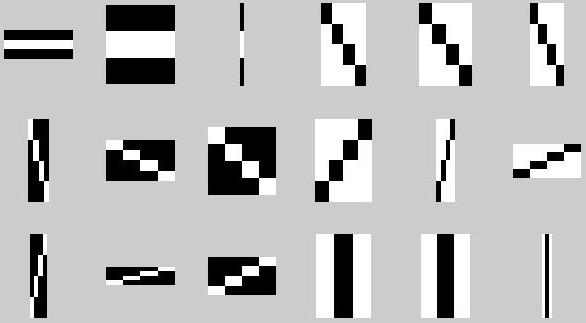
\includegraphics[width=0.45\textwidth]{img/patterns.jpg}
\caption{Patterns}
\label{patterns}
\end{figure}
	\hspace*{10px}The first step of the algorithm is defining the patterns, that are mainly matrixes of different dimensions containing low and high values for intensity (-1 and 1) -- Figure\ref{patterns} indicates a subset of the patterns used. The algorithm used in the \emph{Viola \& Jones} article was designed to loop over all predefined patterns on each position in the image and convolve the specific region of the image with the patterns using the formula:
\begin{flushleft}
\fontfamily{ccr}\selectfont\small
\textcolor{blue}{\emph{$Value = \sum_x\sum_y Image(y:y+h,x:x+w) .* Pattern$}},\\[5pt]
where: \emph{h} -- the heigh of the pattern\\
\hspace*{28px} \emph{w} -- the width of the pattern 
\end{flushleft}
The resulted values for each pattern and location in the image would, then, be used in \emph{AdaBoost} to train an \emph{SVM} classifier. Taking into account the fact that the set of features generated by the algorithm for each pattern and each image, was extremely large, and the training took too much time. We have decided to use just random locations at which to convolve the patterns with a region of the image (that would have the same size with the pattern). Figure~\ref{Haar_features} indicates what \emph{AdaBoost} would choose as being the most representative 5 features for the front side and rear side of the bills.\\
\begin{figure}[!hbtp]
\centering
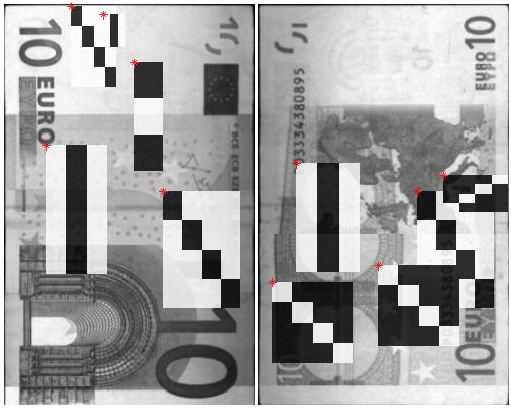
\includegraphics[width=0.45\textwidth]{img/haar.jpg}
\caption{Front and Rear images}
\label{Haar_features}
\end{figure}
	\hspace*{10px}The results obtained using \emph{Haar features} were not as good as we would have expected them to be. An explanation for this may be the fact that the patterns defined were not entirely able to model the dirt present on the bills.\\
	\hspace*{10px}The second approach that we have tried was to define a set of patterns as before, and to segment each image into smaller regions that would be, then, convolved with the patterns. The results obtained using this technique represented the input set of features for the \emph{AdaBoost algorithm}. Figure~\ref{convolved} will help getting a better understanding of how the convolved regions of image and patterns would look like. In this image it is plotted the result obtained when convolving a simple pattern such as: \textbf{[1 -1;-1 1]} with an entire bill.\\
\begin{figure}[!hbtp]
\centering
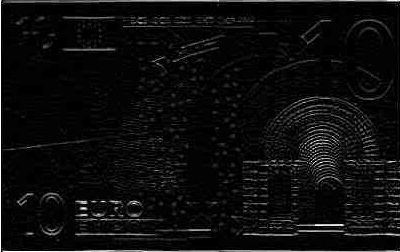
\includegraphics[width=0.45\textwidth]{img/convolution.jpg}
\caption{Convolution of an entire bill with a simple pattern}
\label{convolved}
\end{figure} 
Thus, the resulted set of models would represent the input features used in \emph{AdaBoost}. For establishing the set of the best \emph{T} features we have tried using both \emph{SVM} and \emph{Gaussian distribution}, and the results retrieved by the last one seemed slightly better than the ones obtained while using \emph{SVM}. In the case in which \emph{SVM} was used, a model was generated for each available feature. This model would give the best separation between the values corresponding to that feature for fit images and those for unfit images. In the case of the \emph{Gaussian distribution}, the mean and covariance of features corresponding to fit images were computed, respectively the mean and covariance for the features corresponding to unfit images. The predicted class was defined by using the \todo{\emph{MAP} (maximum aposterior probability) estimation}. The formula for computing the maximum aposterior probability for fit, respectively unfit class is given by:
\begin{flushleft}
\fontfamily{ccr}\selectfont\small
\textcolor{blue}{
$argmax_{\theta_{fit}}P(\theta_{fit}\mid X) = $\\[3pt]
\hspace*{70px}$\frac{P(\theta_{fit})*P(X\mid \theta_{fit})}{P(\theta_{fit})*P(X\mid \theta_{fit}) + P(\theta_{unfit})*P(X\mid \theta_{unfit})}$\\[5pt]
$argmax_{\theta_{unfit}}P(\theta_{fit}\mid X) = $\\[3pt]
\hspace*{70px}$\frac{P(\theta_{unfit})*P(X\mid \theta_{unfit})}{P(\theta_{fit})*P(X\mid \theta_{fit}) + P(\theta_{unfit})*P(X\mid \theta_{unfit})}$\\[5pt]}
where:
\begin{itemize}
\item $P(\theta_{fit}), P(\theta_{unfit})$ -- marginal probabilities of "fit" class, respectively "unfit" class
\item $\theta_{fit}, \theta_{unfit}$ -- the parameters of the classes (mean and covariance) 
\item $P(X\mid \theta_{fit}),P(X\mid \theta_{unfit})$ -- the conditional probabilities of the two classes (representing normal distributions)
\end{itemize}
\end{flushleft}
	\hspace*{10px}The available image set was spilt into a holdout set and the rest of the data was applied for training the final model using the random sub-sampling cross-validation technique, which was repeated several times. The whole process was also repeated a number of times to ensure a correct estimation of the predictions. For each round of the cross-validation, a model was trained using the \emph{AdaBoost algorithm} described above. The obtained model was, then, tested by building the strong classifier and computing the corresponding values for: \emph{true-positive estimation}, \emph{true-negative estimation}, \emph{false-positive estimation} and \emph{false-negative estimation}. In Figure~\ref{nr_models} is depicted the plot of the accuracy of the classifiers for front and rear corresponding to different numbers of features chosen to be used in the final strong classifier.\\ 
\begin{figure}[!hbtp]
\centering
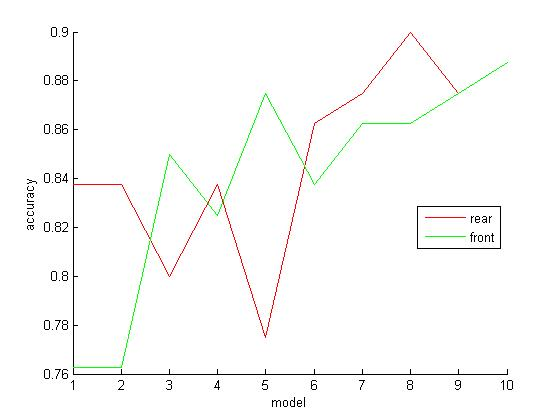
\includegraphics[width=0.45\textwidth]{img/nr_features.jpg}
\caption{Accuracy/number of features for rear and front classifiers}
\label{nr_models}
\end{figure}
 		\hspace*{10px}In this approach we have used two classifiers: one for the rear side and another for the front side of the bills and the predictions given by the two classifiers were combined into a third one using Naive Bayes.\\
		\hspace*{10px}In order to create the final model, we have tried two different methods: 
\begin{itemize}
\item the first one was essentially just choosing the best model (the one that gives the minimum error) throughout all the repetitions and all the rounds in the cross-validation;
\item the second method was to use a system of voting -- each time a feature was chosen by the \emph{AdaBoost} algorithm, it would receive a vote. In the end the top \emph{T} most voted features throughout all the cross-validation rounds and all the repetitions would be chosen from the best model found. The corresponding weights would be generate by taking the mean of the features\rq\@ $\alpha$-weights computed in the \emph{AdaBoost} algorithm;     
\end{itemize}
As we would have expected, the second method for defining the best model, proved to give better results in this case so it was chosen to be applied.\\
\section{Implementation}\label{sec:implementation}
		\begin{algorithm}[!hbtp]
			\caption{AdaBoost learning features}
			\label{AdaBoost}
			\begin{algorithmic}[1]
			\medskip
			\STATE \tbf{function} AdaBoostLearn($T$, $M$, $S$) 
			\STATE {$T$ = nr. of hypothesis}
			\STATE {$M$ = Models}
			\STATE {$S$ = training-set, \{$(x_1,y_1),...(x_n,y_n)$\} \\ with $x_i \epsilon X$ and $y_i \epsilon \{-1, 1\}$ }
			\STATE {$D_{1(i)} \leftarrow \frac{1}{n}$, with $i=1,...,n$}
			\FOR {$t=1$ to $T$}
				\STATE {$error_t \leftarrow 0$}
				\FOR {$m \epsilon M$}
					\STATE {$h_j(x_i) \leftarrow predict(x_i)$ \%\tit{svm or gaussian distribution}}
					\STATE {$error_j \leftarrow \sum^n_{i=1}D_t(i)[y_i \neq h_j(x_i)]$}
					\IF {$error_j < error_t$}
						\STATE {$error_t \leftarrow error_j$}
						\STATE {$h_t \leftarrow h_j$}
					\ENDIF
				\ENDFOR
				\STATE {$\alpha_t \leftarrow 0.5 \cdot \log{\frac{1-error_t}{error_t}}$}
				\FOR {$i=1$ to $n$}
					\STATE {$D_{t+1}(i) \leftarrow \frac{D_t(i)\exp{-\alpha_t \cdot y_i \cdot h_t(x_i)}}{Z_t}$}
				\ENDFOR
			\ENDFOR
			\STATE {\tbf{return} $\alpha, h$}
			\end{algorithmic}
			\label{alg:AdaBoostLearn}
		\end{algorithm}
		\begin{algorithm}[!hbtp]
			\caption{AdaBoost Prediction}
			\label{AdaBoost_pred}
			\begin{algorithmic}[1]
			\medskip
			\STATE \tbf{function} AdaBoostPredict($\alpha$, $h$, $I$)
			\STATE { $\alpha$ = weights }
			\STATE { $h$ = weak classifiers}
			\STATE {$I$ = image}
			\STATE {$p$ = prediction} 
			\FOR {$t=1$ to $length(\alpha)$}
				\STATE $p \leftarrow p + \alpha_th_t(I)$
			\ENDFOR
			\STATE {\tbf{return} $sign(p)$}
			\end{algorithmic}
			\label{alg:AdaBoostPredict}
		\end{algorithm}

	\section{Results}\label{sec:results}

	\section{Conclusion}\label{sec:conclusion}

	\begin{thebibliography}{2}
		\bibitem{Haar}
			P. Viola \& M. Jones:\\
			\tit{Rapid Object Detection using a Boosted Cascade of Simple Features}
			(CVPR 2001)
		\bibitem{Ada}
			AdaBoost: \\
			\tit{http://en.wikipedia.org/wiki/AdaBoost}	
	\end{thebibliography}

\end{document}
